%------------------------------------------------------------------------------%
%                                   cholesky                                   %
%------------------------------------------------------------------------------%

\clearpage{}
\section{Cholesky}

The initial tasks undertaken during the project was the implementation of the
Cholesky decomposition. The work that will be described in this section has been
realized to demonstrate the capabilities of \gls{hh}, and it has been done
without any knowledge of how \gls{fds} operates. For these reasons, we will
describe this work before explaining the principles of the simulator.\\

\gls{fds}'s simulation requires solving equations. For this, they use the
Cholesky algorithm, however, their current implementation is not fast enough. In
this section, we will start by presenting the algorithm. Then we will explain
the implementation with \gls{hh} before presenting the results. For the
measurements, our implementation will be compared to the OpenBLAS's
implementation as it is one of the fastest currently available.

\subsection{The algorithm}
\label{sec:choalgo}

The Cholesky algorithm is used to solve systems of linear equations of the form
$Ax = y$, where $A \in M_{n,n}(\mathrm{R})$ is symmetric and positive-definite
\cite{choleskywiki}. The principle is to decompose the matrix $A$ into a matrix
$L$ such that $A = LL^{T}$, where $L \in M_{n,n}(\mathrm{R})$ is a lower
triangular matrix. We then solve the two sub-problems: $Lx' = y$ and $L^{T}x =
x'$.

There are several ways to implement this algorithm. Here, we are going to
implement the block version since it is the most suited for parallel computing.
Indeed, one most of the important concepts of \gls{hpc} is optimizing CPU cache
usage. To achieve this, we will decompose our matrix into smaller blocks that
can be entirely loaded into the cache, minimizing the need for the CPU to access
the RAM.

The version of the algorithm that we will use is described in
\cite{choleskyblock}. This algorithm proceeds in three steps. First, consider
the matrix $A$ shown in the figure \ref{fig:chodeca}. In this figure, $D$
represents a diagonal block, $C$ is a column (composed of multiple blocks) and
$A'$ is a sub-matrix.

% [Cholesky decomposition] {{{
\begin{figure}[!ht]
  \begin{center}
    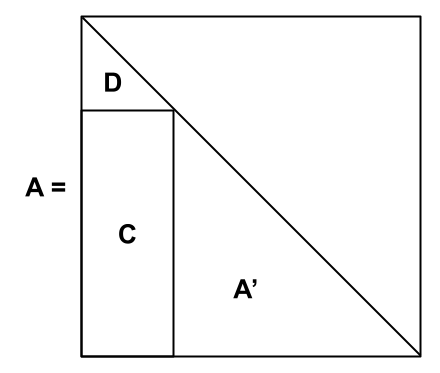
\includegraphics[scale=0.4]{img/cho-img/cho_block_dec_A.png}
    \caption{Cholesky decomposition: matrix A}
    \label{fig:chodeca}
  \end{center}
\end{figure}
%}}}

The first step of the algorithm is to process the diagonal element $D$. To do
this, we use the sequential version of the algorithm. It will be fast enough
given the size of the block. The second step is to update the elements on the
column beneath the diagonal block. To do this, we solve the system
$C_{\text{new}} = C(D^{T})^{-1}$. Once this is done, we have computed the first
column of the result matrix $L$. The final step consists of updating the rest of
the matrix $A$ by performing $A' = A' - CC^{T}$.

Once we have obtained the matrix $L$, we can proceed to the solving part to find
the solutions of the system. This process can be decomposed in two steps: first,
we solve the equation involving the diagonal block, then we update the rest of
the matrix and the result vector using the partial solution (we remove the
variables from the equation). We repeat these steps for each diagonal block to
solve a sub-problem. The solver must be applied twice to solve the two
sub-problems $Lx' = y$ and $L^{T}x = x'$.

\subsection{Implementation}

The implementation of the algorithm was done in two parts. The decomposition was
implemented first, and once it was fully functional, the solver part has been
added. This approach was chosen because the decomposition is the most critical
part of the algorithm. It was important to compare our version with the
OpenBLAS's one before implementing the solver.

The first implementation of the decomposition involved creating a graph that
followed the steps described in the section \ref{sec:choalgo} similarly to
OpenBLAS. This graph is shown in the figure \ref{fig:chograph}.

% [Cholesky decomposition graph] {{{
\begin{figure}[!ht]
  \begin{center}
    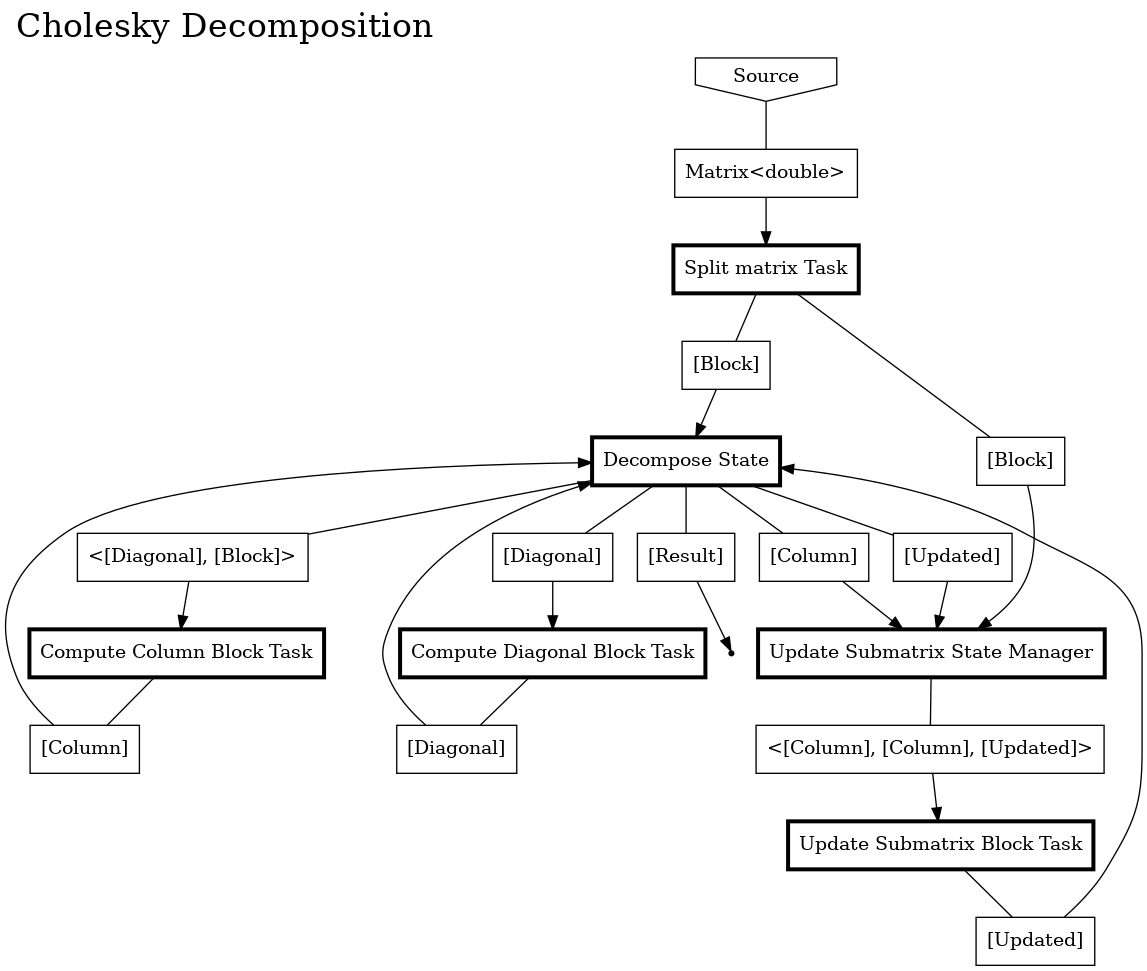
\includegraphics[scale=0.3]{img/cho-img/decompose_graph.png}
    \caption{Cholesky decomposition graph}
    \label{fig:chograph}
  \end{center}
\end{figure}
%}}}

In this diagram, tasks and states are represented by the bold rectangles and the
data by the regular rectangles. There are two kinds of data that flow into this
graph. The first kind is the \texttt{Matrix} that is the input of the graph and
the second kind is the matrix blocks represented by the block's identifier
enclosed in \texttt{'[]'}. The matrix is given to the \texttt{Split Task}, which
generates the blocks. The blocks have identifiers, which define their types.
These identifiers are used to send the right blocks to the appropriate task (or
state). For instance, when the \texttt{Decompose State} sends a
\texttt{Diagonal} block, it is transferred to the \texttt{Compute Diagonal Block
Task}. The execution of this graph can be visualized as follows:

\begin{enumerate}
  \item Split the matrix into blocks (\texttt{Split Matrix Task}).
  \item Compute the diagonal element \textbf{C} (\texttt{Compute Diagonal Block Task}).
  \item Compute the elements on the column \textbf{D} (\texttt{Compute Column Block Task}).
  \item Update the sub-matrix \textbf{A'} (\texttt{Update State / Task}).
  \item Restart from 2 with the blocks of \textbf{A'} (and send the result
    blocks).
\end{enumerate}

This first solution was too slow because the three steps were executed
sequentially (which is also what is done in OpenBLAS). By doing so, we were
loosing a lot of parallelism. For instance, the computation of the diagonal
elements could be done with only one thread and all the other threads had to
wait. To optimize the algorithm, we aimed to keep the threads as busy as
possible, and the solution for this was to rely on early computation by
processing the blocks as soon as they are ready. For instance, we can begin
solving the next diagonal element before all the blocks of the sub-matrix $A'$
are updated. Similarly, we can handle the column the same manner.

To make the early computation possible, the block's data structure was modified.
A \texttt{rank} attribute was added to keep track of the modifications on
the blocks. Each time a block is updated, its rank is incremented. When the rank
of a block is equal to its column number, it is ready to be processed, and it is
processed when its rank is superior to its column number. The states use pending
lists to store indices of blocks that should be processed, and iterate on these
lists to launch the computation of all ready blocks. The graph maintains the
same structure, but the operations in the state have been drastically changed.

In this second version, several verifications are required, using the rank
in the states. Furthermore, both of the states have a vector of block pointers
that are shared between them to make sure that when the \textit{decompose state}
changes a rank, the \textit{update state} can be aware of the modification
directly, without any notification. This improves the performances but adds
complexity in the states.

Eventually, we managed to have good performances with this second version as
OpenBLAS does not make any early computation. We will present our results in the
section \ref{sec:chores}.

For the solver, we use a second graph that is employed twice to solve the two
sub-systems of the matrix. The graph is shown in the figure
\ref{fig:solvergraph}.

% [Solver graph] {{{
\begin{figure}[!ht]
  \begin{center}
    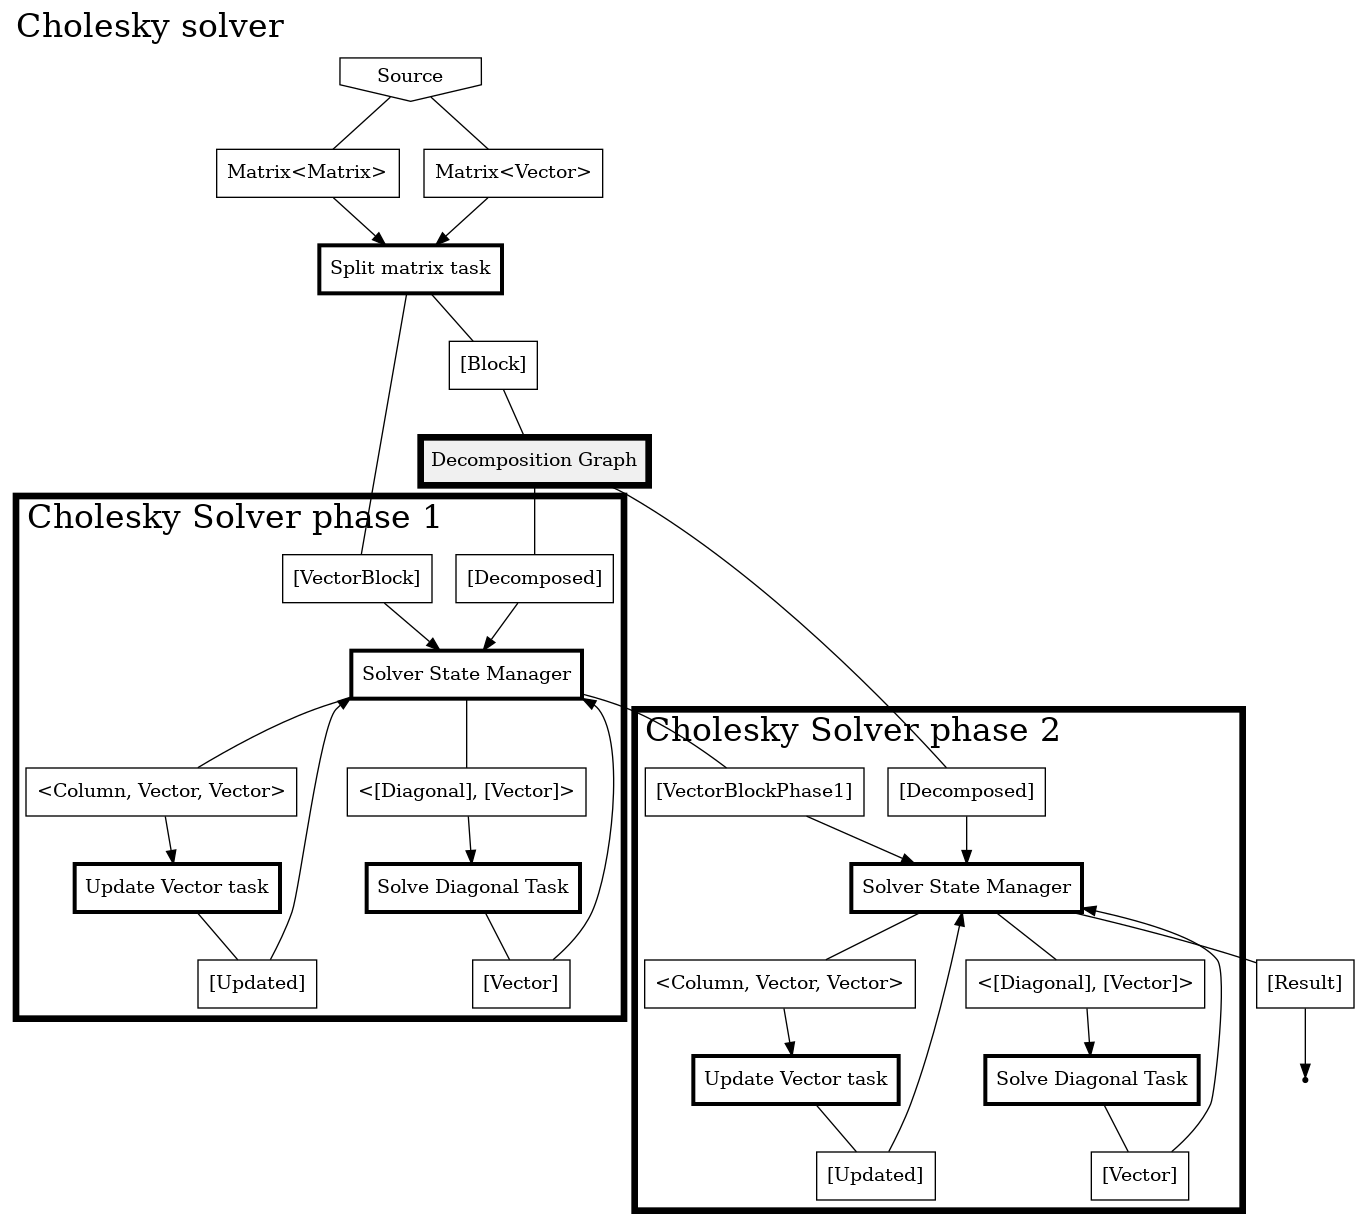
\includegraphics[scale=0.2]{img/cho-img/solver_graph.png}
    \caption{Solver graph}
    \label{fig:solvergraph}
  \end{center}
\end{figure}
%}}}

Here, we observe that there are two sub-graphs for the solving part. These two
graphs solve the two sub-problems that we described earlier. The first solver is
directly connected to the decomposition graph, and it receives the decomposed
block. Both solver graphs are connected to the split task, and they receive the
split vector blocks.

In this graph, we use the same matrix blocks as in the decomposition graph,
allowing us to start the solving part directly when the decomposition graph
outputs the first result block. The hole principle of \gls{hh} is to allow the
creation of pipelines in which the data flows continuously, so we avoid having
unnecessary barriers\footnote{Points in the program where we must wait for the
completion of task before starting the next one.} in the process. Here, we do
not have to finish the decomposition entirely to start solving the blocks. This
helps to maintain maximal parallelism and ensure the computer's resources are
used efficiently. In other words, if we represented the computation time between
the logical cores in a Gantt chart, our goal would be to optimize the overlap
between tasks and minimize gaps as much as possible (the cores should not be in
a wait state for too long, at all ideally).

\clearpage{}
\subsection{The results}
\label{sec:chores}

Now that we have explained the algorithm and its implementation, we will analyse
the results of the measurements on the decomposition algorithm using both the
OpenBLAS's implementation and the \gls{hh}'s one. Two sets of measures have been
made on a cluster node with 192 CPU cores. For the first set, the problem size
was 40,000 and the program has been run with a maximum of
256 threads. On the second set, we used a 100,000 matrix and a maximum of
384 threads (utilizing all the cores). For each problem, we measured the
computation times of the two algorithm for different number of threads (from
1 to the maximum) in order to see the relative speedup. With \gls{hh}, the
number of threads was changed only for the most critical task (the update
task). It was fixed to the optimal numbers for the other tasks (these
numbers were found by doing first tests measures beforehand).\\

First, let us analyse the measurements made on the 40,000 matrix. The figure
\ref{fig:40000graph} shows the graph generated at the end of the program using
\gls{hh}'s profiling tool. Here we can see that the bottleneck of the program is
indeed the update task as we have explained before. We can see as well that only
one thread was allocated to the diagonal task and 12 were allocated to the
column task. The diagonal task does not require more than one thread since it
processes at most one block at a time (this is shown by the maximum queue size
\texttt{MQS} on the rectangle before the task). For the column task, it appears
relatively slow (as indicated by the color). We could put more threads on it, but
we have to make sure that we keep enough resources for the update task.

% [Hedgehog graph for the 40000 matrix] {{{
\begin{figure}[!ht]
  \begin{center}
    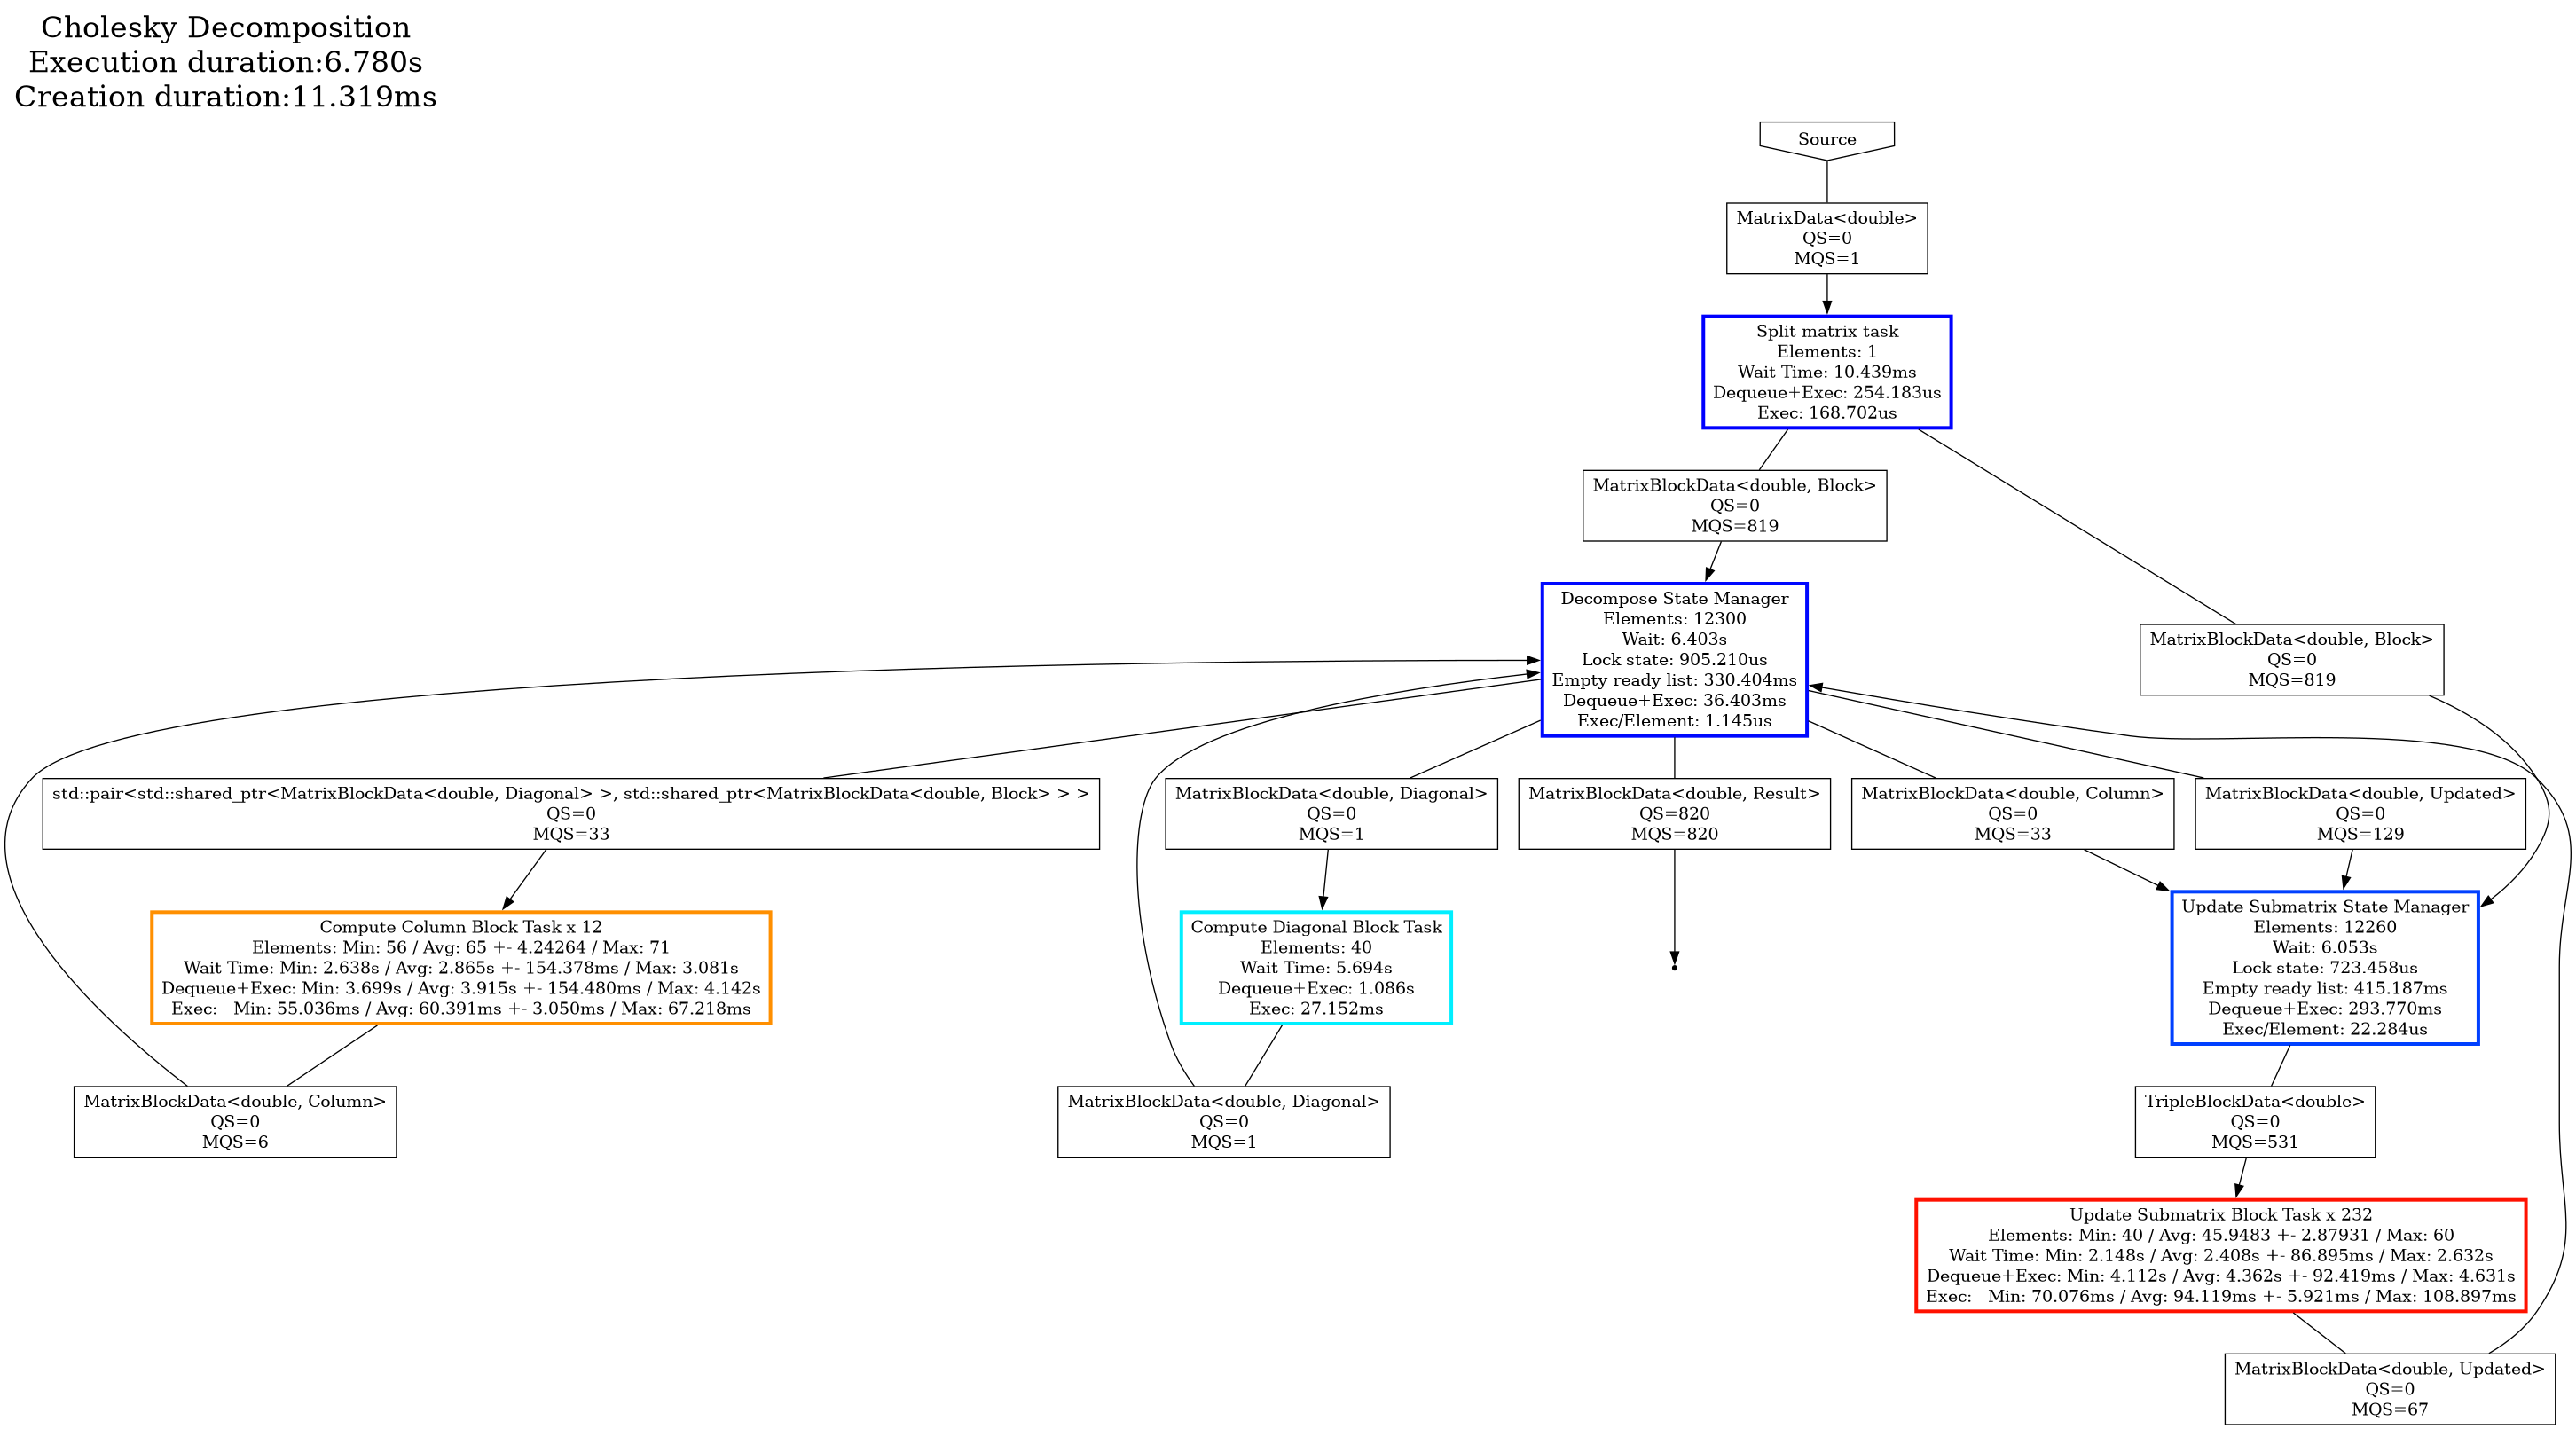
\includegraphics[scale=0.15]{img/cho-img/40000.png}
    \caption{Hedgehog graph for the 40000 matrix}
    \label{fig:40000graph}
  \end{center}
\end{figure}
%}}}

On the figures \ref{fig:time40000} and \ref{fig:speedups40000} we see the
computation times of the two implementations and the speedup of the \gls{hh}'s
version compared to the OpenBLAS's one for the 40000 matrix. Here, an
interesting behavior is observed for the OpenBLAS program. As the number threads
increases, the \gls{hh} program continues to scale, while the OpenBLAS's one
become unstable around a hundred threads. A possible explanation is that
OpenBLAS is optimized for non-hyper-threaded configurations. For these
measurements, we allocated 256 threads on the cluster which means that we
could have used 1 thread per core till more than 128 threads was allocated to
the program. This number is quite to the point where the instability begins to
appear on the OpenBLAS's measurements.

\begin{figure}[!htb]
  \begin{minipage}{0.48\linewidth}
    \centering
    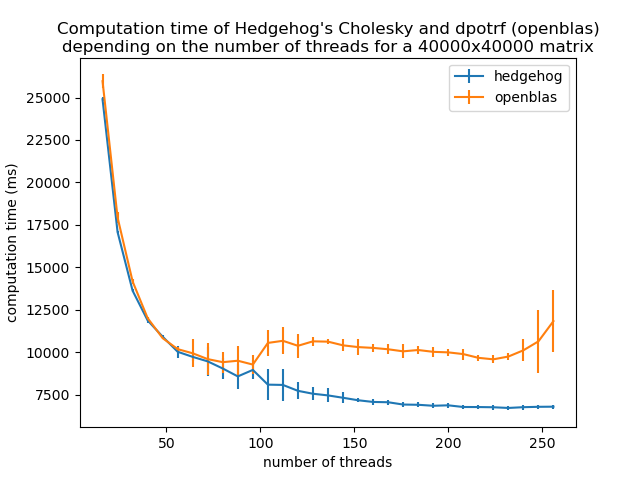
\includegraphics[scale=0.5]{img/cho-img/times-40000.png}
    \caption{Computation times for a 40000 matrix}
    \label{fig:time40000}
  \end{minipage}\hfill
  \begin{minipage}{0.48\linewidth}
    \centering
    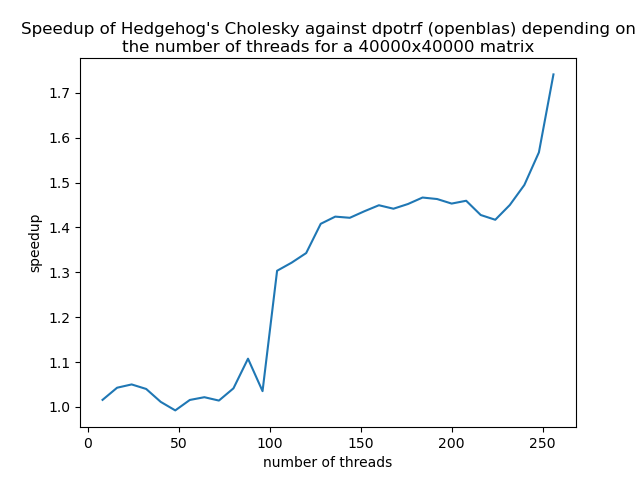
\includegraphics[scale=0.5]{img/cho-img/speedup-40000.png}
    \caption{Speedups for a 40000 matrix (hedgehog / OpenBLAS)}
    \label{fig:speedups40000}
  \end{minipage}
\end{figure}

The figure \ref{fig:relativespeedup40000} shows the relative speedup for each
program ($\frac{time_{one_thread}}{time_{n_thread}}$). As we can see, neither
program achieves a significant speedup. This can be attributed to the fact that
the current problem is too small, limiting resource utilisation. For this
reason, we conducted more measurements with a bigger problem.

% [Relative speedups for a 40000 matrix] {{{
\begin{figure}[!ht]
  \begin{center}
    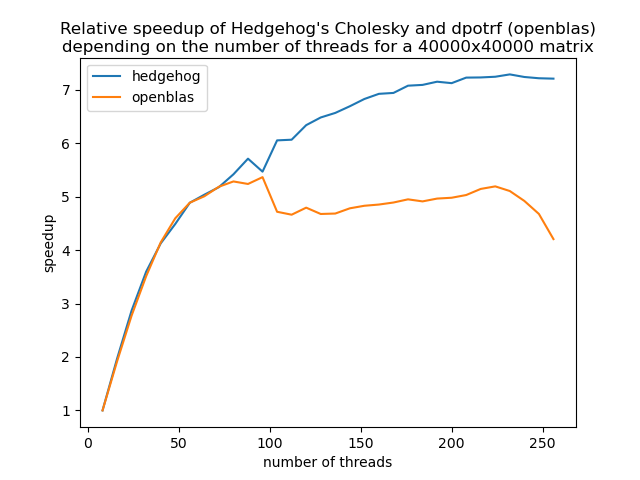
\includegraphics[scale=0.8]{img/cho-img/relative-speedup-40000.png}
    \caption{Relative speedups for a 40000 matrix}
    \label{fig:relativespeedup40000}
  \end{center}
\end{figure}
%}}}

The second set of measurements used a 100,000 by 100,000 matrix, and utilized up
to 384 threads. The figures \ref{fig:time100000} and \ref{fig:speedups100000}
show the computation times of the two implementations as well as the speedup
of \gls{hh} against OpenBLAS as observed previously. These two plots shows
similar results than the previous ones.

\begin{figure}[!htb]
  \begin{minipage}{0.48\linewidth}
    \centering
    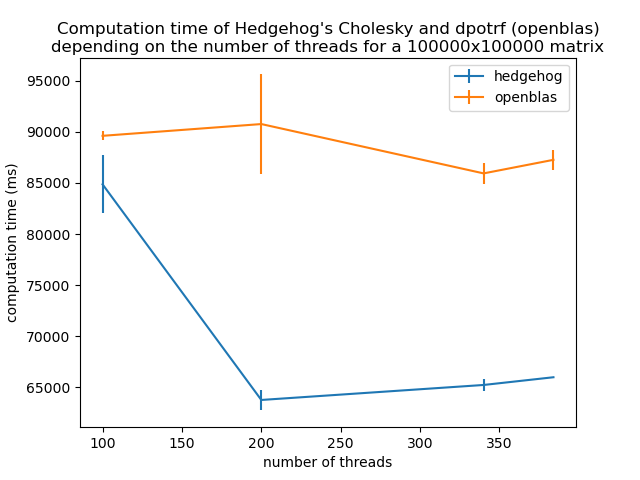
\includegraphics[scale=0.5]{img/cho-img/times-100000.png}
    \caption{Computation times for a 100000 matrix}
    \label{fig:time100000}
  \end{minipage}\hfill
  \begin{minipage}{0.48\linewidth}
    \centering
    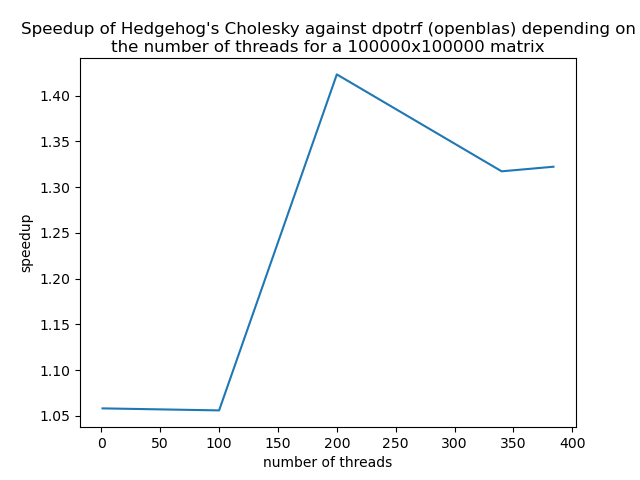
\includegraphics[scale=0.5]{img/cho-img/speedup-100000.png}
    \caption{Speedups for a 100000 matrix (hedgehog / OpenBLAS)}
    \label{fig:speedups100000}
  \end{minipage}
\end{figure}

The figure \ref{fig:relativespeedup100000} shows that we have a way better
relative speedup for the two algorithms. This means that the resources are
better exploited with a bigger problem.

% [Relative speedups for a 100000 matrix] {{{
\begin{figure}[!ht]
  \begin{center}
    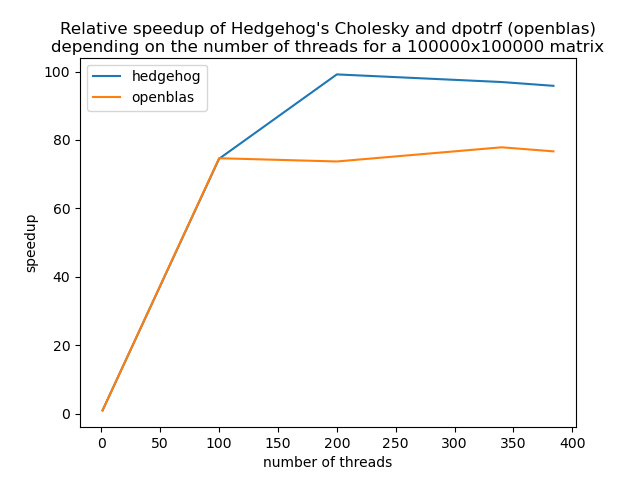
\includegraphics[scale=0.8]{img/cho-img/relative-speedup-100000.png}
    \caption{Relative speedups for a 100000 matrix}
    \label{fig:relativespeedup100000}
  \end{center}
\end{figure}
%}}}

Eventually, we achieved to have better performances than OpenBLAS by
incorporating more early computation. Additionally, the program remains readable
and easy to understand. This demonstrates the effectiveness of the data-flow
graph approach is in parallel computing, as well as the capabilities of the
\gls{hh} library.
